%% In the documentclass line, replace "noanswers" with "answers" to view the key.

\documentclass[noanswers]{exam}
\usepackage[utf8]{inputenc}

\title{Learning Activity 19}
\author{Chapter 13}
\date{STAT 3090}

\usepackage[bottom=2.2cm, left=2.2cm, right=2.2cm, top=2.2cm]{geometry}
%\usepackage[paperheight=11in, paperwidth=17in, margin=1in]{geometry}
\usepackage{dsfont}
\usepackage{amsmath}
\usepackage{amssymb}
\usepackage{amsthm}
\usepackage{array}
\usepackage{stmaryrd}
\usepackage{pgfplots}
\pgfplotsset{width=10cm,compat=1.9}
\usepackage{multicol}
\setlength{\columnsep}{1in}
\usepackage{nicefrac}

\usepackage{multirow}
\usepackage{enumitem}[shortlabels]
\usepackage{tabu}
\definecolor{purp}{RGB}{102,0,204}
\usepackage{tabularx}
\newcolumntype{C}{>{\centering\arraybackslash $}X<{$}}
\usepackage{wrapfig}
\usepackage[export]{adjustbox}


\makeatletter
\pagestyle{headandfoot}
\firstpageheader{\@date}{\@title}{\@author}
\firstpageheadrule
\runningfootrule
\runningfooter{}{\thepage\ / \numpages}{\@title}
\makeatother

\newcommand{\abs}[1]{\left|#1\right|}
\newcommand{\mat}[4]{\left( \begin{tabular}{>{$}c<{$} >{$}c<{$}} #1&#2 \\ #3&#4 \end{tabular} \right)}
\newcommand{\msc}[1]{\mathds{#1}}
\newcommand{\Z}{\mathds{Z}}
\newcommand{\R}{\mathds{R}}
\newcommand{\N}{\mathds{N}}
\newcommand{\Q}{\mathds{Q}}
\newcommand{\C}{\mathds{C}}
\newcommand{\so}{\implies}
\newcommand{\set}[2]{\left\{ #1 \:|\: #2 \right\}}
\newcommand{\bso}{\Longleftarrow}
\newcommand{\ra}{\rightarrow}
\newcommand{\gen}[1]{\left\langle #1 \right\rangle}
\newcommand{\olin}[1]{\overline{#1}}
\newcommand{\Img}[1]{\text{Im}\left(#1\right)}
\newcommand{\llra}{\longleftrightarrow}
\newcommand{\lra}{\longrightarrow}
\newcommand{\xra}[1]{\xrightarrow{#1}}
\newcommand{\wo}{\setminus}
\newcommand{\mcal}[1]{\mathcal{#1}}
\newcommand{\Aut}[1]{\text{Aut}\left(#1\right)}
\newcommand{\Inn}[1]{\text{Inn}\left(#1\right)}
\newcommand{\syl}[2]{\text{Syl}_{#1}(#2)}
\newcommand{\norm}[1]{\left\|#1\right\|}
\newcommand{\infnorm}[1]{\left\|#1\right\|_{\infty}}
\newcommand{\xn}{\{x_n\}}
\newcommand{\sig}{\sigma}
\newcommand{\id}{\text{id}}
\newcommand{\ep}{\epsilon}
\newcommand{\st}{\text{ s.t. }}
\newcommand{\ran}[1]{\text{Ran}(#1)}
\newcommand{\nCr}[2]{\binom{#1}{#2}}
\newcommand{\Exr}[1]{\paragraph{Exercise #1:}}
\newcommand{\pg}{\paragraph{}}
\newcommand{\ulin}[1]{\underline{#1}}
\newcommand{\tc}[1]{\textcolor{purp}{#1}}

% Solution Specs
\unframedsolutions
\renewcommand{\solutiontitle}{}
\SolutionEmphasis{\color{purp}}
\CorrectChoiceEmphasis{\color{purp}\bfseries}
\setlength\fillinlinelength{1.5in}
\renewcommand{\arraystretch}{2}


\begin{document}
\noindent\begin{tabular}{@{}p{1.4in}p{5.2in}@{}}
Group Member Names: & \hrulefill
\end{tabular}

\vspace{1mm}
\noindent If you have group members who collaborated but were not logged into the Zoom session, please note in the submission comments how they collaborated on the learning activity.

\vspace{5mm}

\noindent A major airline wishes to determine if it can predict the elapsed time of a flight delay in minutes, $y$, using the distance of the flight to the destination in miles, $x$. Simple linear regression was performed in JMP for a large sample of 29,009 delayed flights gathered during the previous year. (See the JMP dataset \verb|Airline Delays.jmp|.) Use the output below to answer the questions in this Learning Activity.

\begin{multicols}{2}
	\noindent \textbf{Scatter Plot of Elapsed Time vs.\ Distance}
	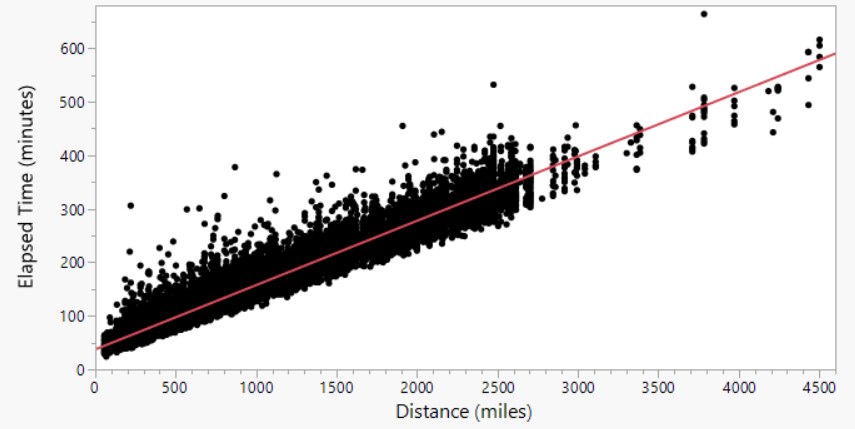
\includegraphics[scale=.55]{STAT_3090_LA19_scatter-plot.PNG}
	\begin{flushright}
	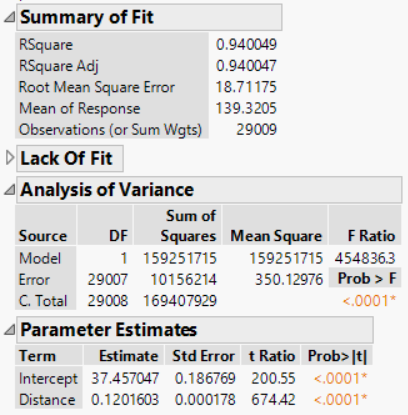
\includegraphics[scale=.75]{STAT_3090_LA19_linear-regression.PNG}
	\end{flushright}
\end{multicols}

\begin{questions}	
	
	\question Write the equation for the \textbf{least squares regression line} in terms of $x$ and $\hat{y}$, where $x=$ distance of the flight (in miles) and $\hat{y}=$ estimated elapsed time of the delay (in minutes).
		
	\begin{solution}[\stretch{1}]

	\vspace{1mm}
	
	$\hat{y}=37.457047+0.1201603x$
	
	\vspace{1mm}
	
	\end{solution}
	
	\question Interpret the \textbf{slope} of the estimated regression equation in context of the problem.
	
	\begin{solution}[\stretch{1}]
	
	\vspace{1mm}
	
	$b_1=0.1201603$. For every additional mile of flight distance, the elapsed delay time will increase on average by 0.1202 minutes.
	
	\vspace{1mm}	
	
	\end{solution}
	
	\question Is there a valid interpretation of the \textbf{$y$-intercept} in context of the problem? If so, interpret the $y$-intercept. If not, explain why.
	
	\begin{solution}[\stretch{1}]
	
	\vspace{1mm}
	
	$b_0=37.457047$. There is no valid interpretation of the $y$-intercept in this context because it does not make sense to have a flight of $x=0$ miles long.
	
	\vspace{1mm}
	
	\end{solution}
	
	\question Interpret the \textbf{standard error} of prediction found by your regression analysis. Include units.
	
	
	\begin{solution}[\stretch{1}]
	
	\vspace{1mm}
	
	$s=18.71175$ minutes. For any given flight distance, the true elapsed delay time will vary from the predicted delay time on average by approximately 18.7 minutes.
	
	\vspace{1mm}
	
	\end{solution}	
	
\end{questions}
%-----------------------------------------------------------------------------%

\end{document}
